%=========================================================================
% Member 4 sections: 3.1, 3.3, 3.6, 3.7, 5.2
% This file is generated by code/_sync_sections.py -- edit the
% sections/member4_<n>.tex files instead, then re-run the sync script.
% Requires in preamble (add alongside existing \usepackage lines):
%   \usepackage{booktabs}   % also fixes the current \toprule compile error
%   \usepackage{url}        % \url in the bibliography (also missing upstream)
%=========================================================================

% Member 4 - Section 3.1 Overall Framework
\subsection{Overall Framework}
\label{sec:overall_framework}

Fig.~\ref{fig:framework} summarizes the pipeline. All three experimental groups share one architecture, one set of data splits, and one evaluation protocol, and differ in exactly one factor: the set of images used for training.

\begin{figure}[t]
\centering
% Overall framework diagram. Source: figures/framework.mmd (Mermaid).
% Render with:  npx -y @mermaid-js/mermaid-cli -i figures/framework.mmd -o figures/framework.pdf -b white -s 2
% If the PDF is absent, fall back to the PNG, and finally to a placeholder.
\IfFileExists{figures/framework.pdf}{%
  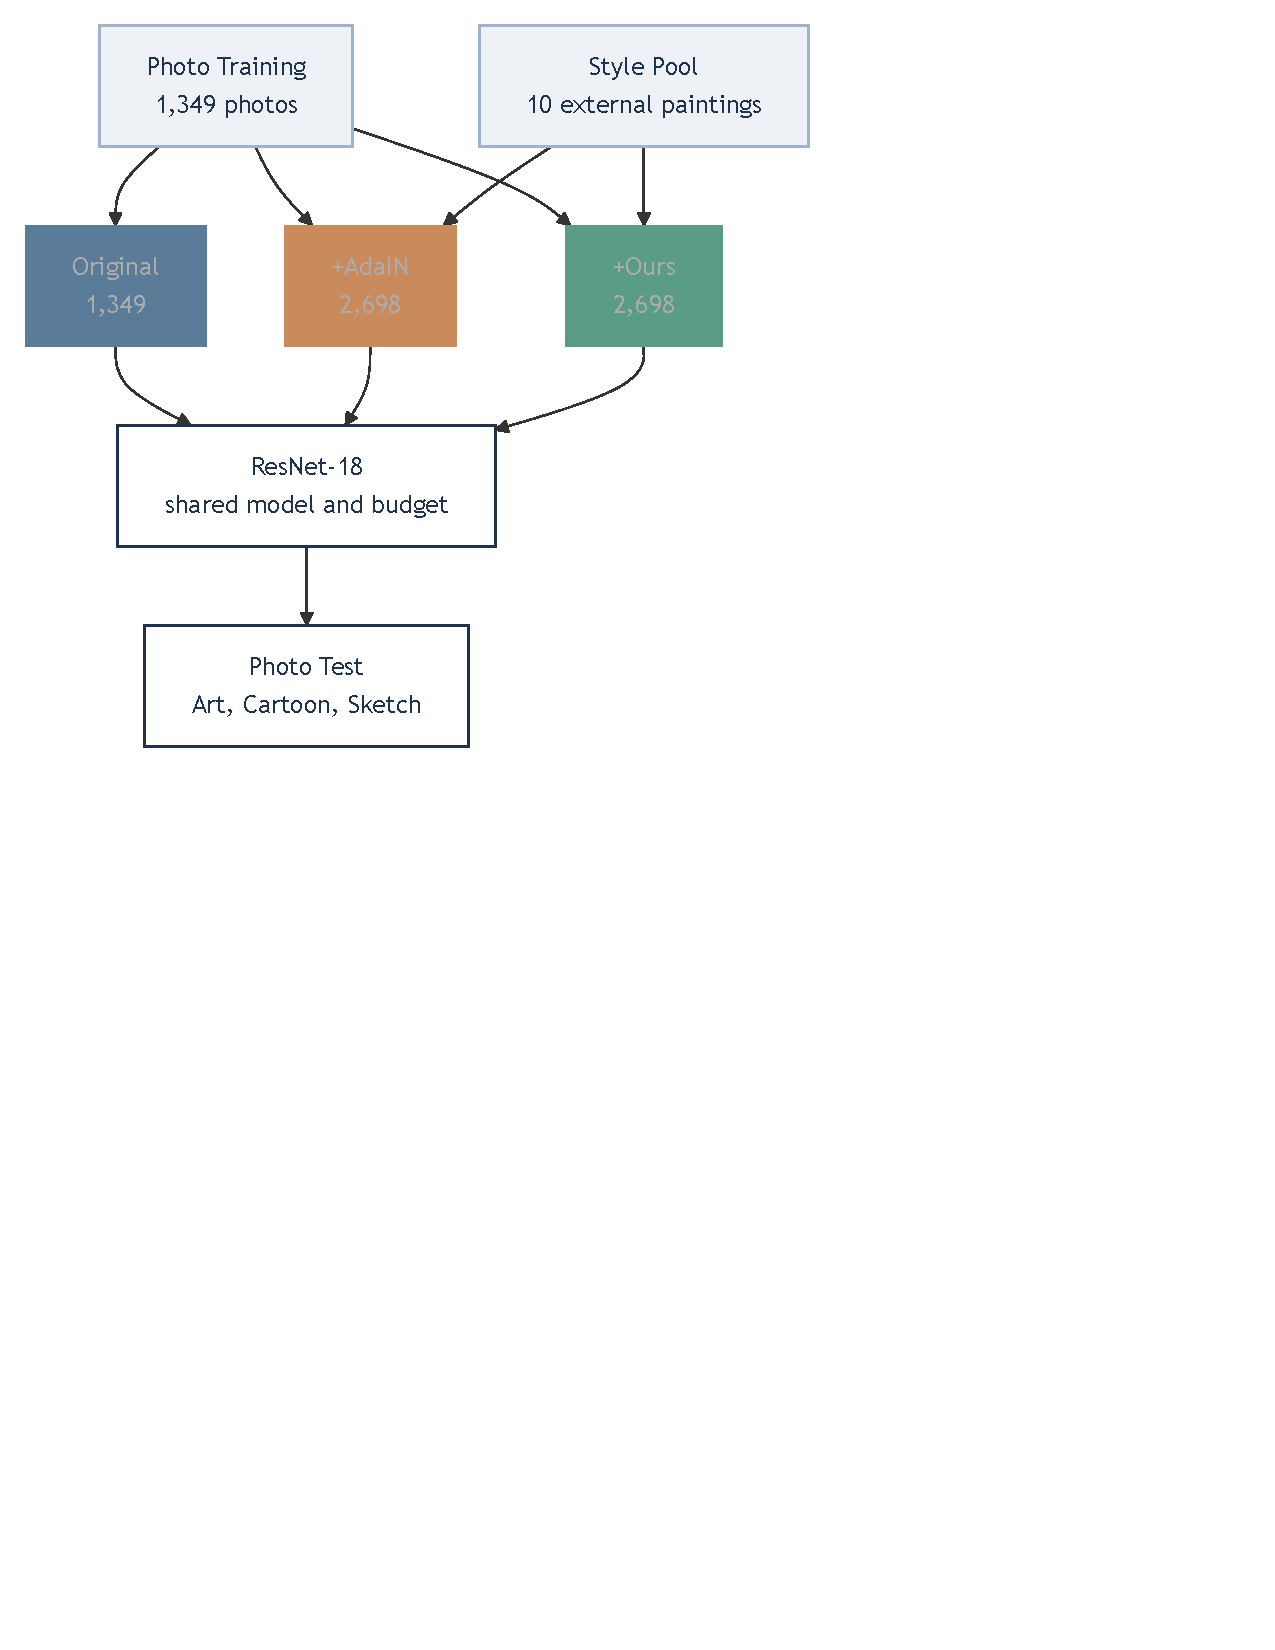
\includegraphics[width=\columnwidth]{figures/framework.pdf}%
}{%
  \IfFileExists{figures/framework.png}{%
    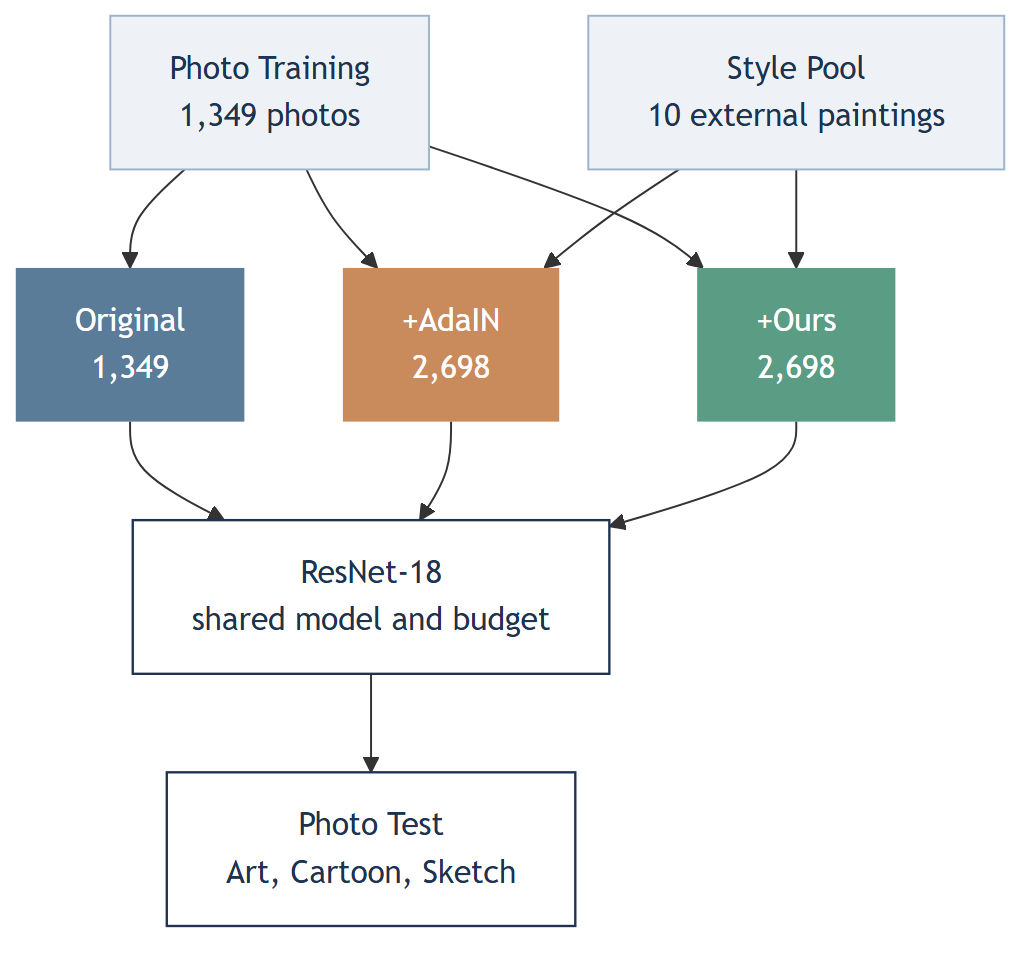
\includegraphics[width=\columnwidth]{figures/framework.png}%
  }{%
    \fbox{\parbox[c][2.2cm][c]{\dimexpr\columnwidth-2\fboxsep-2\fboxrule\relax}{\centering Placeholder: overall framework figure (planned).}}%
  }%
}
\caption{Overall framework. Photo Training images feed three training sets: originals only, originals plus AdaIN stylizations, and originals plus structure-preserving stylizations. Both stylized sets draw their style references from one frozen pool of external paintings. A single ResNet-18 training and evaluation protocol is applied to all three groups.}
\label{fig:framework}
\end{figure}

Stylized training images are produced \textit{offline}. Member 2's AdaIN generator and member 3's structure-preserving generator each write images to disk together with a manifest that records the content image, the style image, the style strength $\alpha$, and, for the structure-preserving variant, the structure parameter $\beta$. Training then reads from these fixed manifests, so the three groups go through an identical data-loading path. Nothing about the stylization is recomputed or resampled during classifier training, which keeps the classifier-side training code common to all groups.

Table~\ref{tab:groups} defines the three groups. The comparison Original vs.\ +AdaIN isolates the value of added style diversity (experiment 2), and +AdaIN vs.\ +Ours isolates the value of structure preservation (experiment 3), as detailed in Section~\ref{sec:exp_design}.

\begin{table}[t]
\caption{The three training groups. All groups use the same splits, model, and evaluation.}
\label{tab:groups}
\centering
\small
\setlength{\tabcolsep}{4pt}
\begin{tabular}{@{}lrr@{}}
\toprule
Group & Training images & Composition \\
\midrule
Original & 1{,}349 & Photo Training only \\
+AdaIN   & 2{,}698 & $+ 1{,}349$ AdaIN \\
+Ours    & 2{,}698 & $+ 1{,}349$ structure-preserving \\
\bottomrule
\end{tabular}
\end{table}

%==================================================

% Member 4 - Section 3.3 ResNet-18 Baseline
\subsection{ResNet-18 Baseline}
\label{sec:resnet_baseline}

We use ResNet-18~\cite{he2016resnet} as the classifier for all groups. It is the standard backbone for PACS-style domain generalization studies, and its moderate size fits our single-GPU compute budget while leaving room for multi-seed replication.

The network is initialized with ImageNet-pretrained weights, and the final fully connected layer is replaced with a seven-way classifier head. All layers are fine-tuned jointly. Pretraining matters in our setting: Photo Training has only 1{,}349 images, and training the same architecture from scratch on this amount of data yields a weak baseline that would compress the dynamic range of all comparisons.

\textit{Input transforms.} Training uses RandomResizedCrop to $224\times224$ with scale $(0.7, 1.0)$ and a horizontal flip, followed by ImageNet normalization. Evaluation resizes the shorter side to 256, center-crops to $224\times224$, and applies the same normalization. We deliberately exclude photometric augmentation such as color jitter and grayscale: those transformations change style-related statistics, which is exactly the variable under study, so adding them to all groups would confound the comparison. Geometric augmentation only is applied, identically in all groups.

\textit{Optimization.} All groups are trained with SGD (momentum 0.9, weight decay $5\times10^{-4}$, label smoothing 0.1~\cite{szegedy2016rethinking}), initial learning rate 0.01, batch size 64, and a cosine schedule~\cite{loshchilov2017sgdr} over a budget of 30 passes over each group's own training set (Section~\ref{sec:exp_design}). We report the \textit{final} checkpoint of that budget, with no checkpoint selection on any validation split: we measured that selecting on Photo Validation accuracy inflates the seed-to-seed spread of cross-domain accuracy, and the measurement is reported in Section~\ref{sec:training_prep}. Target-domain test sets never influence training, checkpoint selection, or any hyperparameter choice.

% TODO (Member 2): \subsection{AdaIN Style Augmentation}
% TODO (Member 3): \subsection{Structure-Preserving Style Augmentation}

%==================================================

% Member 4 - Section 3.6 Evaluation Metrics
\subsection{Evaluation Metrics}
\label{sec:evaluation_metrics}

\textit{Classification accuracy.} We report top-1 accuracy on Photo Test (in-domain) and on each of Art Painting, Cartoon, and Sketch (cross-domain). The primary metric is the unweighted average of the three cross-domain accuracies. Every configuration is run with three training seeds; we report mean and standard deviation over seeds, and per-domain breakdowns are included so that effects which appear in only one domain are visible.

\textit{Structure preservation.} To characterize the generated data rather than the classifier, we compare each stylized image with its content image using two measures. The first is LPIPS~\cite{zhang2018lpips}, a perceptual distance between the two images; larger values mean the stylization moved the image further from its content. The second is \textbf{EdgeScore}, an edge-consistency measure built from Canny edge maps~\cite{canny1986}. Writing $E_c$ and $E_s$ for the binary edge maps of the content and the stylized image, we report

\[
\text{EdgeScore} = \frac{2PR}{P+R}, \quad
P = \frac{|E_c \cap E_s|}{|E_s|}, \quad
R = \frac{|E_c \cap E_s|}{|E_c|},
\]

which is the F1-style overlap of the two edge maps: it is 1 when the stylized image reproduces all of the content's contours and falls as the stylization erases them. Note that this is an \textit{overlap}, not a difference: it is the harmonic mean of the fraction of stylized edges that coincide with a content edge (precision) and the fraction of content edges that survive in the stylized image (recall). A plain edge difference would score a stylization that adds many spurious edges but keeps the content's contours as poorly as one that erases them, whereas EdgeScore rewards agreement in both directions. Canny thresholds are held fixed across all images so that scores are comparable. These metrics describe how much structure the generated data removes; they are analysis metrics and do not enter training or model selection.

%==================================================

% Member 4 - Section 3.7 Experimental Design and Fair Comparison
\subsection{Experimental Design and Fair Comparison}
\label{sec:exp_design}

\textit{Experiments.} Five experiments answer the research questions in the Introduction. Experiment 1 trains the Original group and measures the Photo-versus-target gap. Experiment 2 compares Original against +AdaIN. Experiment 3 compares +AdaIN against +Ours with everything else held fixed. Experiment 4 sweeps the style strength $\alpha \in \{0.25, 0.5, 0.75, 1.0\}$ for both augmentation methods, tracing the relation between stylization strength, structure preservation, and cross-domain accuracy. A $\beta$ ablation for the structure-preserving method is planned alongside Experiment 4 (Section~5.3). Experiment 5 is the control that makes Experiment 3 interpretable: it isolates the effect of the \emph{spatial} modulation from the effect of the \emph{overall style strength}, which the two differ in simultaneously.

\textit{Why a strength control is necessary.} The structure-preserving map is $\alpha(x,y) = \alpha_0(1-\beta M)$, so wherever $M$ is large the applied strength is necessarily below $\alpha_0$. The spatial map therefore always carries \emph{less} total style than a uniform AdaIN at the same $\alpha_0$: at our main setting ($\alpha_0 = 0.5$, $\beta = 0.7$) its mean is $0.374$, against $0.500$ for the uniform mix. A direct comparison of +AdaIN against +Ours consequently changes two things at once---the spatial modulation and the overall style strength---and a difference in accuracy cannot be attributed to either alone. We resolve this with two additional controls, both trained under the identical protocol:

\begin{itemize}
\item \textit{Strength-matched uniform AdaIN.} A plain uniform AdaIN whose strength is, for each image individually, the mean of that image's spatial $\alpha$ map. It has the same total style energy as the spatial map and differs from it only in that the strength is not modulated in space.
\item \textit{Equal-strength spatial map.} The $\alpha_0$ is recalibrated so that the spatial map's mean is exactly $0.500$, matching the uniform AdaIN at $\alpha = 0.5$ to four decimals: with $\beta = 0.7$ and $\overline{M} = 0.361$, this requires $\alpha_0 = 0.500 / (1 - 0.7 \times 0.361) = 0.6692$. Here +Ours and +AdaIN differ in the spatial modulation and in nothing else.
\end{itemize}

Both controls use the same style pool, the same frozen content--style pairing, the same seeds, the same step budget, and the same classifier, and both are verified by the fairness checker before training.

\textit{Fairness controls.} Because the compared methods differ only in their training images, the following quantities are fixed across groups:

\begin{itemize}
\item \textit{Same original data:} all groups train on the identical 1{,}349 Photo Training images from Table~\ref{tab:splits}.
\item \textit{Same style pool:} both augmented groups draw style references from one frozen pool of 10 style images, fixed with a content-hash manifest before any training run. The pool holds external paintings that are not part of PACS, and the checker verifies this mechanically (the ``No test-set leakage'' item below).
\item \textit{Same augmentation count:} each augmented group adds exactly one stylized image per original training image (1{,}349 added images).
\item \textit{Same content--style pairing:} the style image paired with each content image is drawn once with a fixed seed and reused by both generators, so the only difference between the two augmented datasets is the stylization algorithm itself.
\item \textit{Same transform pipeline and classifier:} one training script, one transform definition, one ResNet-18 configuration for all groups.
\item \textit{Same optimization budget:} all groups receive the same number of \emph{passes over their own training set}, 30 epochs at batch size 64, so the step budget is $S = 30\lceil N/64\rceil$ for a group with $N$ training images ($S = 660$ for the Original group, $S = 1{,}290$ for the augmented groups). The epoch count is held fixed rather than the step count, so a group with a larger training set is not under-trained relative to one with a smaller one. Validation is evaluated at the same step cadence for every group.
\item \textit{Same evaluation and seeds:} all groups use the test lists of Table~\ref{tab:splits} and are run with seeds $\{0, 1, 2\}$.
\item \textit{No checkpoint selection:} the reported model is the final checkpoint of the step budget, for every group and every seed. This removes a selection step that we measured to be harmful (Section~\ref{sec:resnet_baseline}).
\item \textit{No test-set leakage:} the style pool is built from external paintings and contains no PACS image. Because Art Painting, Cartoon, and Sketch are the evaluation domains, a style reference drawn from any of them would place the test appearance into the training set. The checker compares the content hash of every style image against the whole local PACS copy and rejects the run if any style image is a PACS image.
\item \textit{Fairness verification.} A checker script validates these constraints mechanically before training: it confirms that the augmented manifests contain the same original images, the same style pool hash, the same augmentation count, that the content--style pairing is identical in both manifests, that no style image is a PACS image, and that the training configuration fingerprint is identical across groups. The configuration fingerprint is recomputed from the full training configuration recorded in each run summary, so a run whose hyper-parameters differ is rejected. A run that fails any check is excluded from results.
\end{itemize}

\textit{Reporting.} Table~\ref{tab:results} shows the result table format used throughout. Entries are mean$\pm$standard deviation over three seeds. Differences between groups are reported per seed, so that a gain which depends on one favorable seed is visible rather than hidden in the average. Because all groups share the same seeds, the design is \emph{paired}, and we report paired $t$ tests with 95\% confidence intervals rather than independent-samples tests; at three seeds this is the more powerful choice, and it is the only honest one at this sample size.

\begin{table}[t]
\caption{Result table. Entries are mean$\pm$standard deviation over three training seeds (final checkpoint of the 30-epoch budget over each group's own training set). The last two rows are the controls that separate the effect of the spatial modulation from the effect of the overall style strength.}
\label{tab:results}
\centering
\scriptsize
\setlength{\tabcolsep}{2.0pt}
\begin{tabular}{@{}lccccc@{}}
\toprule
Training method & Photo & Art & Cartoon & Sketch & Avg \\
\midrule
Original & $99.0\pm0.3$ & $63.2\pm3.7$ & $25.1\pm1.8$ & $31.5\pm4.2$ & $39.9\pm2.7$ \\
+AdaIN   & $99.2\pm0.3$ & $69.0\pm0.7$ & $32.2\pm1.7$ & $40.2\pm1.3$ & $\mathbf{47.1\pm0.8}$ \\
+AdaIN (matched) & $99.4\pm0.0$ & $68.0\pm1.3$ & $29.7\pm1.2$ & $38.4\pm2.5$ & $45.4\pm0.3$ \\
+Ours    & $99.8\pm0.3$ & $68.5\pm0.6$ & $30.0\pm0.9$ & $36.7\pm3.9$ & $45.1\pm1.5$ \\
+Ours (eq.\ strength) & $99.6\pm0.3$ & $68.1\pm0.8$ & $31.1\pm0.3$ & $41.8\pm3.3$ & $\mathbf{47.0\pm0.9}$ \\
\bottomrule
\end{tabular}
\end{table}

Experiment 1 is complete. The Original group reaches $99.0\%$ on Photo Test but only $39.9\%$ averaged over the three unseen domains, so the domain gap is both large and unambiguous. The gap is not uniform: Art Painting, whose appearance is closest to photography, is recognized at $63.2\%$, whereas Cartoon and Sketch, which discard most photographic cues, fall to $25.1\%$ and $31.5\%$. This ordering is the one we would expect from a classifier that relies mainly on photographic texture, and it identifies Cartoon and Sketch as the domains where style augmentation has the most room to help.

Experiment 2 shows that style augmentation itself is effective: adding 1{,}349 AdaIN-stylized images lifts the cross-domain average from $39.9\%$ to $47.1\%$, a gain of $7.2$ points, and it does so while \emph{reducing} the seed-to-seed spread from $2.7$ to $0.8$ points. The variance reduction matters as much as the mean: augmentation does not merely raise the expected accuracy, it makes the outcome reproducible, which is the property a single-seed result cannot show. The gain is consistent across all three target domains and is largest on Sketch ($+8.7$), the domain furthest from the source.

Experiments 3 and 5 give a clear and, we think, more interesting answer than a simple win would have. Against +AdaIN, +Ours does \emph{not} improve accuracy: the paired difference is $-2.0$ points ($t=-3.21$, $p=0.085$) at the main setting and $-0.3$ points ($p=0.81$) against the strength-matched control. The strength-matched control explains why: uniform AdaIN at the same mean strength scores $45.4\%$, i.e.\ $1.8$ points \emph{below} uniform AdaIN at full strength. The accuracy of these groups is governed almost entirely by how much style is applied, not by how that style is distributed in space. The equal-strength spatial map confirms this directly: with the mean strength pinned to $0.500$, it reaches $47.0\%$ against +AdaIN's $47.1\%$, a paired difference of $-0.1$ points ($p=0.89$)---the two methods are indistinguishable once strength is held fixed.

The mechanism itself does work, but not in the way the classification metric can see. Measured on all 1{,}349 images with paired per-image comparison, the spatial map retains more of the content's edge structure than plain AdaIN ($0.344$ against $0.321$, mean difference $+0.023$, 95\% CI $[+0.022, +0.023]$, $p<10^{-290}$), and its perceptual distance to the content is lower ($0.226$ against $0.279$). Against the strength-matched control, however, the difference \emph{reverses} slightly ($-0.003$, $p<10^{-22}$): the uniform mix at equal strength retains marginally more edges than the spatial map. The spatial modulation therefore does not deliver superior edge preservation once the confound is removed; what it does deliver is weaker stylization, and weaker stylization preserves edges for the trivial reason that less styling destroys fewer of them. Consistent with this, the per-image gain over the strength-matched control does not concentrate on structurally dense images (Spearman $\rho = +0.078$ against edge count; $-0.003$ in the dense half against $-0.003$ in the sparse half), so the mechanism the method is designed around is not observable in the images either.

\begin{figure}[t]
\centering
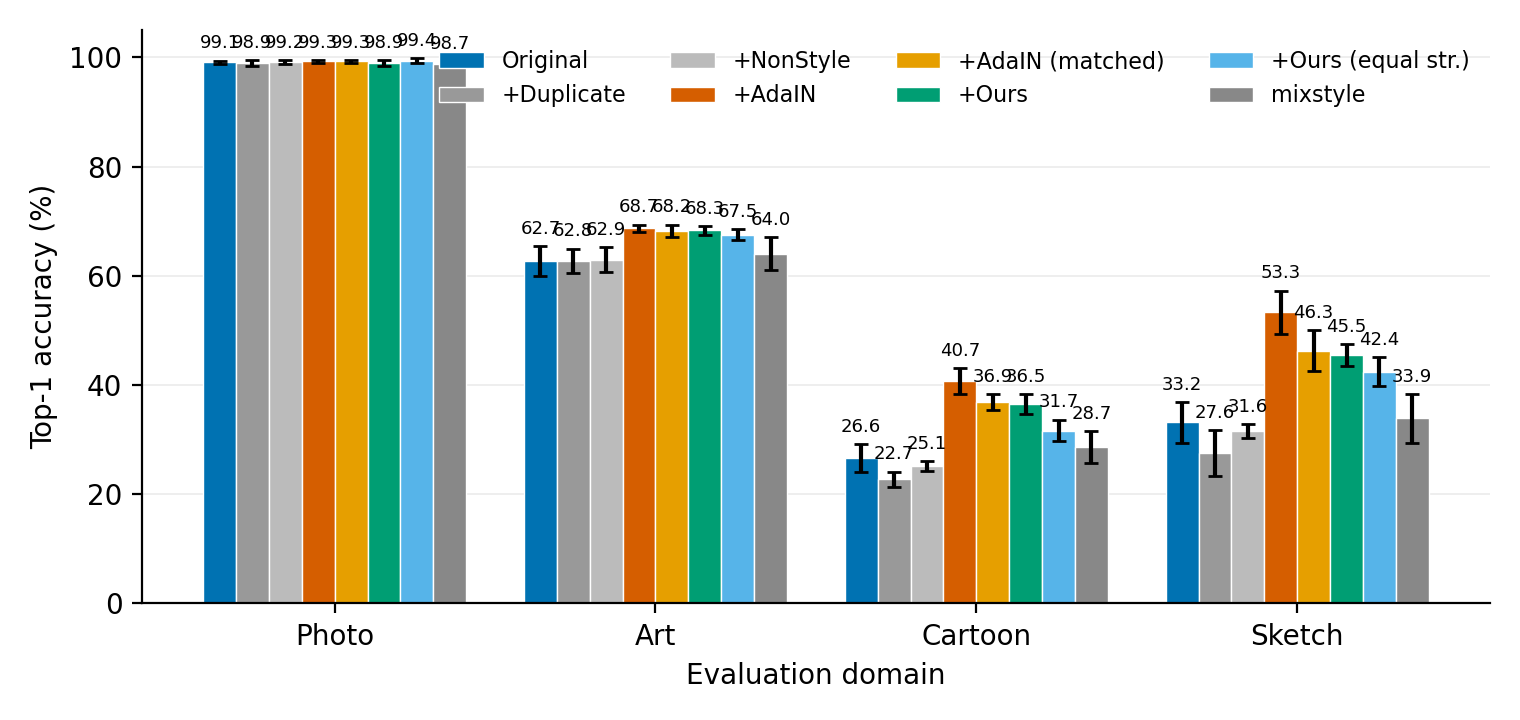
\includegraphics[width=\columnwidth]{figures/results_baseline.png}
\caption{Experiment 1: accuracy of the Original group on the in-domain Photo test set and on the three unseen target domains. Bars are means over three seeds; whiskers are standard deviations.}
\label{fig:results_baseline}
\end{figure}

%==================================================

%==================================================

% Member 4 - Section 5.2 Experiment Completion Plan
\subsection{Experiment Completion Plan}
\label{sec:completion_plan}

The unified training and evaluation code is complete and validated on the local PACS copy, so the remaining experiment work is primarily GPU time. The plan below assumes the two generators are delivered by their owners in week 1; the frozen style pool they will use is already in place (Section~\ref{sec:exp_design}).

\begin{itemize}
\item \textit{Week 1: Experiment 1 and baseline replication.} \textit{Done.} The Original group has been run with seeds $\{0,1,2\}$ on the 660-step budget it retains under the epoch-based protocol, giving $99.0\pm0.3\%$ in-domain and $39.9\pm2.7\%$ cross-domain. A diagnostic run to 1{,}320 steps, recorded but not used for tuning, shows that cross-domain accuracy fluctuates within a narrow band from the first evaluation onwards rather than improving systematically with more steps; the budget was therefore kept at 660 steps for the Original group, and every group reports its final checkpoint (Section~\ref{sec:resnet_baseline}). The budget of the remaining groups was later corrected from a fixed 660 steps to an epoch budget of 30 passes over their own training set, because the fixed budget had given them only 15.7 passes against the Original group's 31.3. The remaining work in this week is to fix the checkpoint-selection policy, which we have done (Section~\ref{sec:resnet_baseline}), and to confirm the final protocol with the group.
\item \textit{Week 2: Experiments 2 and 3.} \textit{Done.} Both augmented datasets were generated from the frozen style pool (1{,}349 images each) and the fairness checker passes on every manifest before training. +AdaIN, +Ours, and both controls have been run with the same three seeds, and the structural metrics (LPIPS, EdgeScore) have been computed on all 1{,}349 images of every dataset.
\item \textit{Week 3: Experiment 4 and ablation.} \textit{In progress.} The $\alpha$ sweep $\{0.25, 0.5, 0.75, 1.0\}$ for both methods is the highest-value remaining item, because our results show that cross-domain accuracy is governed primarily by the overall style strength rather than by the spatial modulation. The $\beta$ sweep for the structure-preserving method follows it. The strength-matched control should be extended to every $\alpha$ in the sweep, so that the strength axis and the modulation axis are separated at every point rather than only at the main setting.
\item \textit{Week 4: Replication and analysis.} The per-domain, per-seed and per-class tables are assembled (Section~\ref{sec:exp_design}). Remaining: failure-case analysis with the $M$ and $\alpha$ maps displayed for images where the method misfires, and the qualitative figure set.
\end{itemize}

Compute budget: one training run takes roughly 10 minutes on the project GPU (RTX 4070 Laptop, 8\,GB), so the full plan above totals approximately 15--20 GPU-hours including sweeps and reruns, which fits the available hardware within the schedule.

% TODO (Member 5): 5.1, 5.4, 5.5

%==================================================

%==================================================


%==================================================
\begin{thebibliography}{00}

\bibitem{zhou2023dgsurvey}
K.~Zhou, Z.~Liu, Y.~Qiao, T.~Xiang, and C.~C.~Loy,
``Domain generalization: A survey,''
\textit{IEEE Trans. Pattern Anal. Mach. Intell.}, vol.~45, no.~4, pp.~4396--4415, 2023.

\bibitem{zhou2021mixstyle}
K.~Zhou, Y.~Yang, Y.~Qiao, and T.~Xiang,
``Domain generalization with MixStyle,''
in \textit{Proc. Int. Conf. Learning Representations (ICLR)}, 2021.

\bibitem{huang2017adain}
X.~Huang and S.~Belongie,
``Arbitrary style transfer in real-time with adaptive instance normalization,''
in \textit{Proc. Int. Conf. Computer Vision (ICCV)}, 2017.

\bibitem{li2017dg}
D.~Li, Y.~Yang, Y.-Z.~Song, and T.~Hospedales,
``Deeper, broader and artier domain generalization,''
in \textit{Proc. Int. Conf. Computer Vision (ICCV)}, 2017.

\bibitem{zhou2020dassl}
K.~Zhou, ``Dassl: Domain adaptation and generalization library,''
\url{https://github.com/KaiyangZhou/Dassl.pytorch}, accessed 2026.

\bibitem{he2016resnet}
K.~He, X.~Zhang, S.~Ren, and J.~Sun,
``Deep residual learning for image recognition,''
in \textit{Proc. IEEE Conf. Computer Vision and Pattern Recognition (CVPR)}, pp.~770--778, 2016.

\bibitem{zhang2018lpips}
R.~Zhang, P.~Isola, A.~A.~Efros, E.~Shechtman, and O.~Wang,
``The unreasonable effectiveness of deep features as a perceptual metric,''
in \textit{Proc. IEEE Conf. Computer Vision and Pattern Recognition (CVPR)}, 2018.

\bibitem{canny1986}
J.~Canny,
``A computational approach to edge detection,''
\textit{IEEE Trans. Pattern Anal. Mach. Intell.}, vol.~8, no.~6, pp.~679--698, 1986.

\bibitem{szegedy2016rethinking}
C.~Szegedy, V.~Vanhoucke, S.~Ioffe, J.~Shlens, and Z.~Wojna,
``Rethinking the Inception architecture for computer vision,''
in \textit{Proc. IEEE Conf. Computer Vision and Pattern Recognition (CVPR)}, 2016.

\bibitem{loshchilov2017sgdr}
I.~Loshchilov and F.~Hutter,
``{SGDR}: Stochastic gradient descent with warm restarts,''
in \textit{Proc. Int. Conf. Learning Representations (ICLR)}, 2017.

\end{thebibliography}

\end{document}
